\documentclass[12pt]{article}
\usepackage[utf8]{inputenc}
\usepackage[english]{babel}
\usepackage{graphicx}
\usepackage{float}
\usepackage{caption}
\usepackage{subcaption}
\usepackage{amsmath}

\setlength{\oddsidemargin}{0in}
\setlength{\evensidemargin}{0in}
\setlength{\textwidth}{6.5in}
\setlength{\topmargin}{-.3in}
\setlength{\textheight}{9in}
\setlength{\parskip}{1em}

% \pagestyle{empty}
\graphicspath{ {images/} }
% ___________________________________________________________________

\begin{document}

\begingroup  
  \centering
  \large Report: Experiments on $\alpha$ updates \par
  \large Arijus Pleska \par
\endgroup
% ___________________________________________________________________

\par The purpose of this report is to assesses whether an auto-regressive topic model is capable to recover the $\alpha$ parameter used in the synthetic data generation process. This report is structured in the following order: at the start, the rationale of the used Bayesian methods are covered; then, the experiment settings are defined; in the next stage, we assess the experiment results; finally, the identified issues are outlined to be discussed during next meeting.
% ___________________________________________________________________

\section*{Preliminaries}
% TODO: Fix the pi expression (remove P(X|...))§

\par In order to understand the experiment settings, it is necessary to be familiar with the auto-regressive and non auto-regressive $\alpha$ priors as well as the Metropolis--Hastings (M--H) algorithm; the expressions of the latter concepts are listed below:
\begin{enumerate}
  \item The auto-regressive $\alpha$ prior:
    \begin{align*}
    p(\alpha_0,\ldots,\alpha_T)=p(\alpha_0)\prod_{t=1}^{T}{p(\alpha_t|\alpha_{t-1})}; \qquad &p(\alpha_t)=f(\alpha_0; 0, \sigma_0^2I), \quad t=0;\\
    & p(\alpha_t)=f(\alpha_t; \alpha_{t-1}, \sigma^2I), \quad t>0.
    \end{align*}
  \item The non auto-regressive $\alpha$ prior:
    \begin{align*}
    p(\alpha_0,\ldots,\alpha_T)=\prod_{t=0}^{T}{p(\alpha_t}); \qquad &p(\alpha_t)=f(\alpha_0; 0, \sigma_0^2I), \quad t \geq 0.
\end{align*}
  \item The rationale of the utilised M--H algorithm variation:\\\\
    For the start, familiarise with the following expressions:
    \begin{align*}
      \dfrac{A(x'|x)}{A(x|x')} = \dfrac{p(x'|x)}{p(x|x')}\cdot \dfrac{q(x'|x)}{q(x|x')} = \dfrac{p(x',x)}{p(x)}\cdot \dfrac{p(x')}{p(x,x')} = \dfrac{p(x')}{p(x)}; \qquad &x' \sim q(x,\delta^2I);\\
      & q = \mathcal{N} \Rightarrow q(x'|x) = q(x|x');
    \end{align*}
    where $x$ is the current state, $x'$ is the proposed state, $A$ is the acceptance distribution, and $q$ is the proposal distribution. Taking the previous results into account, the acceptance rate $r$ is expressed as follows:
    \begin{align*}
      r = \min{\bigg(1, \dfrac{p(x')}{p(x)}\bigg)}.
    \end{align*}
  \item The application of the M--H algorithm to update $\alpha$:\\\\
    Note that the $\alpha$ values are updated independently; that is, the expression for the acceptance rate below is for a single $\alpha$ entry.
    \begin{align*}
      \dfrac{p(z,\alpha^{-tk},\alpha_{t, k}'|X)}{p(z,\alpha|X)} &= \dfrac{p(X|z,\alpha^{-tk},\alpha_{t, k}')\cdot p(z|\alpha^{-tk},\alpha_{t, k}')\cdot p(\alpha^{-tk},\alpha_{t, k}')}{p(X)}\cdot \dfrac{p(X)}{p(X|z,\alpha)\cdot p(z|\alpha)\cdot p(\alpha)}\\
      &= \dfrac{\prod_{k=0}^K\big[\pi(\alpha_{t}')_k^{z_{t,k}}\cdot \pi(\alpha_{t}')_k\big]\cdot p(\alpha_t'|\alpha_{t-1})\cdot p(\alpha_{t+1}|\alpha_t')}{\prod_{k=0}^K\big[\pi(\alpha_t)_k^{z_{t,k}}\cdot \pi(\alpha_{t})_k\big]\cdot p(\alpha_t|\alpha_{t-1})\cdot p(\alpha_{t+1}|\alpha_t)}; \qquad t > 0, \quad t \neq T;
    \end{align*}
    where $\pi$ is the softmax function, $\alpha_{t,k}' \sim \mathcal{N}(\alpha_{t, k}, \delta^2)$, and $\alpha^{-tk}$ denotes $\alpha$ without $\alpha_{t,k}'$; also, for the boundary cases $t=0$ and $t=T$, note that the $p(\alpha)$ term corresponds to $p(\alpha_{0})\cdot p(\alpha_{1}|\alpha_{0})$ and $p(\alpha_{T}|\alpha_{T-1})$ respectively. Further, for computational stability, the previous ratio would be computed in the log space as follows: 
    \begin{align*}
      \log{\bigg[\dfrac{p(z,\alpha^{-tk},\alpha_{t, k}'|X)}{p(z,\alpha|X)}\bigg]} &= \log{\big[p(z,\alpha^{-tk},\alpha_{t, k}'|X)\big]} - \log{\big[p(z,\alpha|X)\big]}; \quad \mbox{where}\\
      \log{\big[p(z,\alpha^{-tk},\alpha_{t, k}'|X)\big]} &=\sum_{k=0}^K\bigg[(z_{t,k}+1)\cdot\log\big[\pi(\alpha_{t}')_k\big]\bigg] + \log\big[p(\alpha_t'|\alpha_{t-1})\big] + \log\big[p(\alpha_{t+1}|\alpha_t')\big],\\
      \log\big[p(z,\alpha|X)\big] &= \sum_{k=0}^K\bigg[(z_{t,k}+1)\cdot\log\big[\pi(\alpha_{t})_k\big]\bigg] + \log\big[p(\alpha_t|\alpha_{t-1})\big] + \log\big[p(\alpha_{t+1}|\alpha_t)\big].
    \end{align*}
    Finally, the acceptance rate is calculated using the formula below.
    \begin{align*}
      r_{t,k} = \exp\bigg[\min{\bigg(0, \log{\bigg[\dfrac{p(z,\alpha^{-tk},\alpha_{t, k}'|X)}{p(z,\alpha|X)}\bigg]}\bigg)}\bigg].
    \end{align*}


    % \begin{align*}
    %   \dfrac{p(\alpha_{t,k}'|\alpha_{t,k})}{p(\alpha_{t,k}|\alpha_{t,k}')}\cdot \dfrac{q(\alpha_{t,k}'|\alpha_{t,k})}{q(\alpha_{t,k}|\alpha_{t,k}')} = \dfrac{p(\alpha_{t,k}',\alpha_{t,k})}{p(\alpha_{t,k})}\cdot \dfrac{p(\alpha_{t,k}')}{p(\alpha_{t,k},\alpha_{t,k}')}, \qquad &\alpha_{t,k}' \sim \mathcal{N}(\alpha_{t,k},\delta^2),\\ 
    %   &q(\alpha_{t,k}'|\alpha_{t,k}) = q(\alpha_{t,k}|\alpha_{t,k})'.
    % \end{align*}
    %   \Rightarrow \dfrac{p(\alpha_{t,k}')}{p(\alpha_{t,k})}

\end{enumerate}


% ___________________________________________________________________

\section*{The Experiment Settings}

\par The intention of the carried experiments is to identify the optimal settings for the Metropolis--Hastings algorithm application. 
The rationale of the carried experiments is based on generating a corpus with pre-defined $\alpha$ changes. Based on the experiments, we will determine which techniques display higher performance in reproducing the pre-defined $\alpha$ fluctuations over time. To expand on the corpus generation settings, the parameters used are listed below:
\begin{itemize}
  \item The number of topics: K = 2;
  \item The number of documents (time slices): T = 20;
  \item The size of vocabulary: V = 10;
  \item The number of words per document t: $N_t \sim \mbox{Pois}(\lambda),\quad \lambda = 1000$.
\end{itemize}
Speaking of $\alpha_k$ development over time (documents), $\alpha_0$ is a sine curve and $\alpha_1$ is a cosine curve; the corresponding topic distributions over documents (i.e., $\theta = \mbox{softmax}(\alpha)$)) are illustrated in Figure 1 below.
\begin{figure}[H]
  \centering
  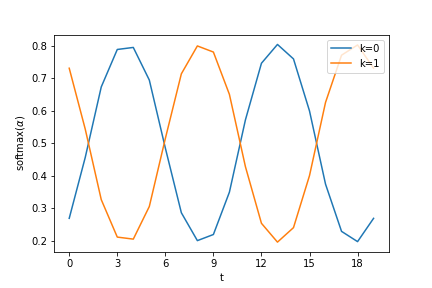
\includegraphics[width=0.5\textwidth]{theta_initial}
  \caption{The values of $\mbox{softmax}(\alpha)$ used in the generative process.}
\end{figure}
Speaking of $\beta$, the parameter was initially pre-defined and kept constant throughout the dynamic generative process; $\beta$ is illustrated in Figure 2 below.
\begin{figure}[H]
  \centering
  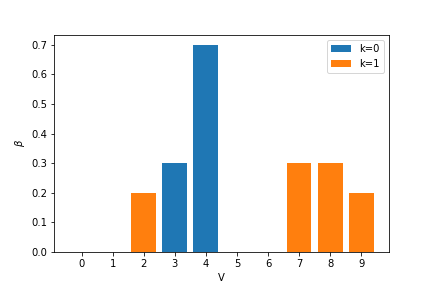
\includegraphics[width=0.5\textwidth]{beta_initial}
  \caption{The values of $\beta$ used in the generative process.}
\end{figure}
% ___________________________________________________________________

\section*{The experiment results}

\par The first experiment is focused on discovering an optimal choice of the variances. Note that the first experiment is carried using the auto-regressive model; therefore, three different types of variances were considered: the `basic' variance $\sigma^2_0$, the `auto-regressive' variance $\sigma^2$, and the `proposed' variance $\delta^2$. 

\par For the first experiment, $\delta^2$ was kept constant and set to $1$. Effectively, low $\delta^2$ values suggest that the convergence of $\alpha$ is slow and stable, whereas for high values of $\delta^2$ the convergence is faster and less stable. In both cases, with a high number of iterations, a low-error $\alpha$ value will be found. Therefore, we are focusing to tune only the $\sigma^2_0$ and $\sigma^2$ variances. Also, note that two visualisation of topic distribution over documents are provided: at 1000 iterations; and at 2000 iterations.

\begin{figure}[H]
  \begin{subfigure}[b]{0.33\textwidth}
    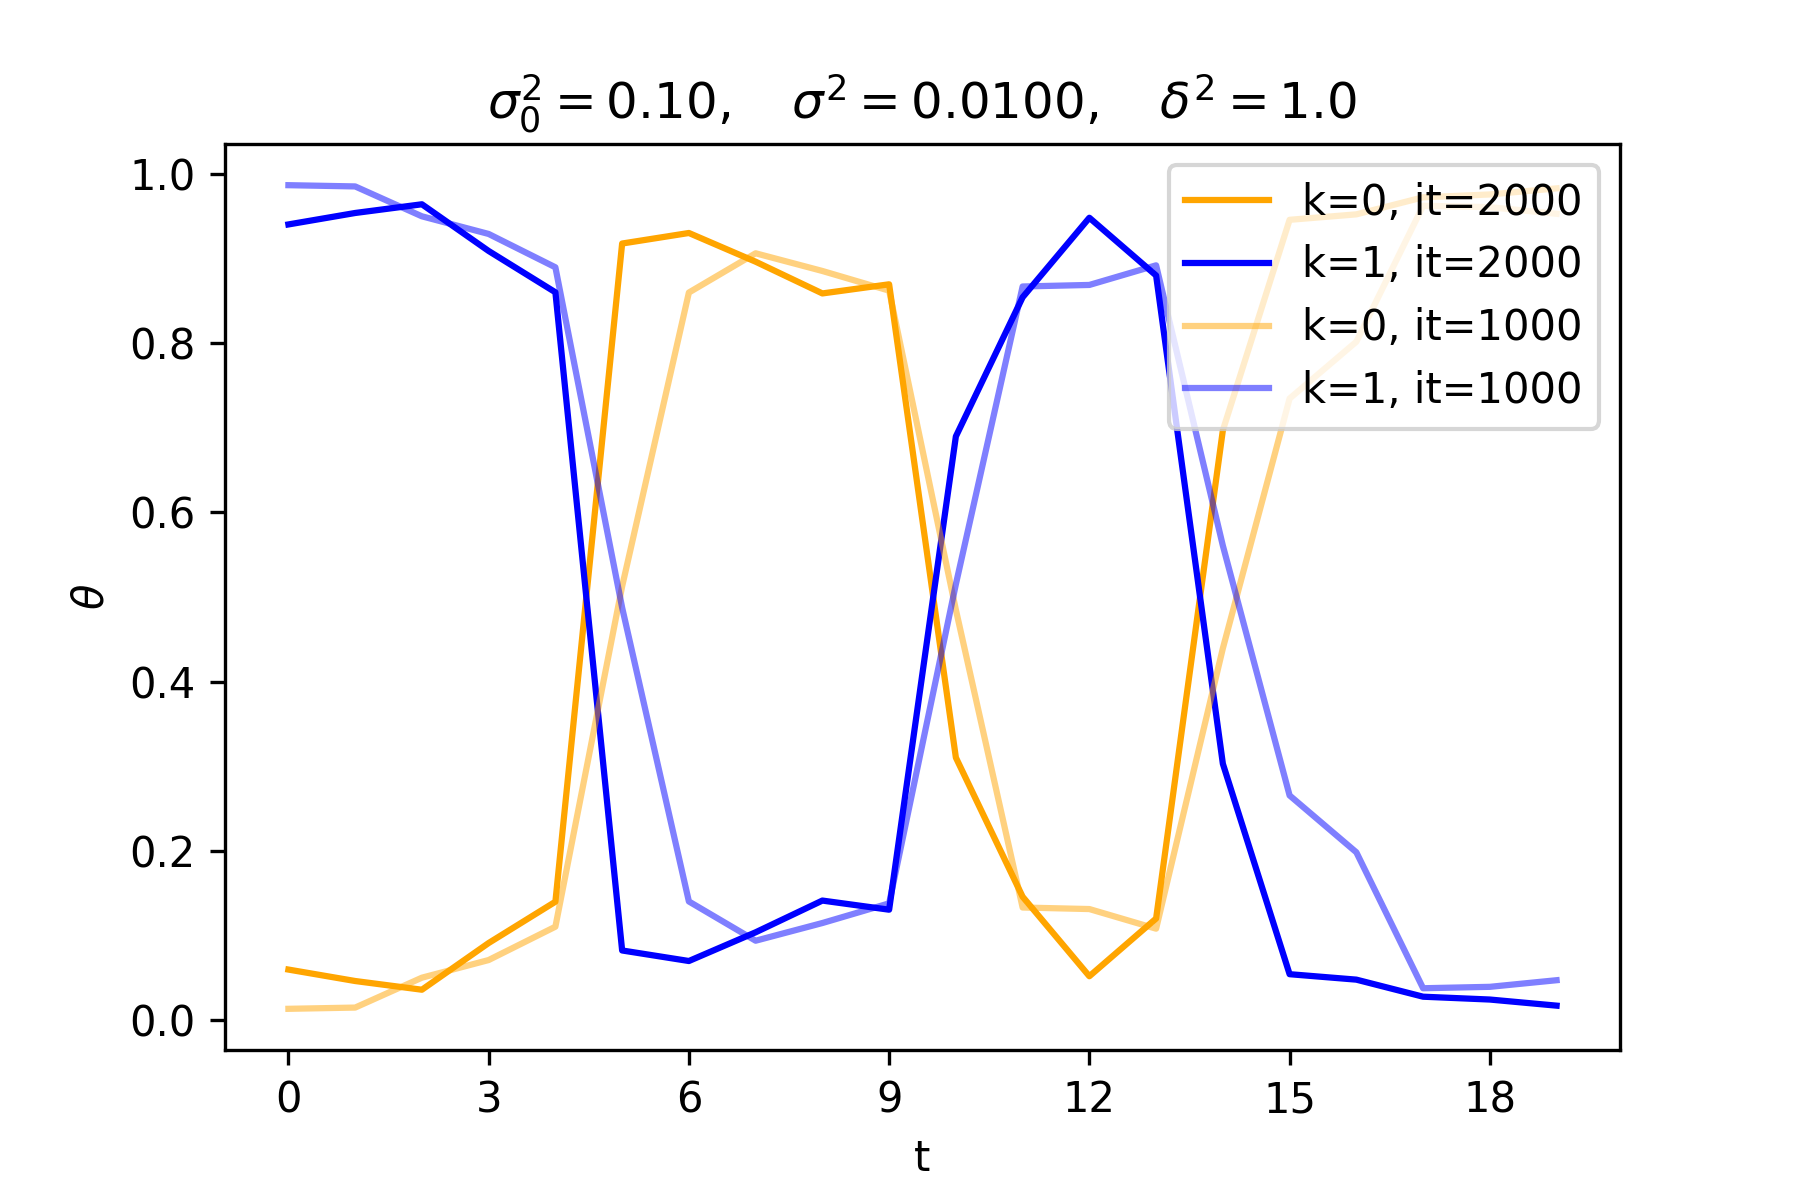
\includegraphics[width=\linewidth]{init_1E-01|basic_1E-02|prop_1E+00|it_2000|autoreg_True}
  \end{subfigure}%
  \begin{subfigure}[b]{0.33\textwidth}
    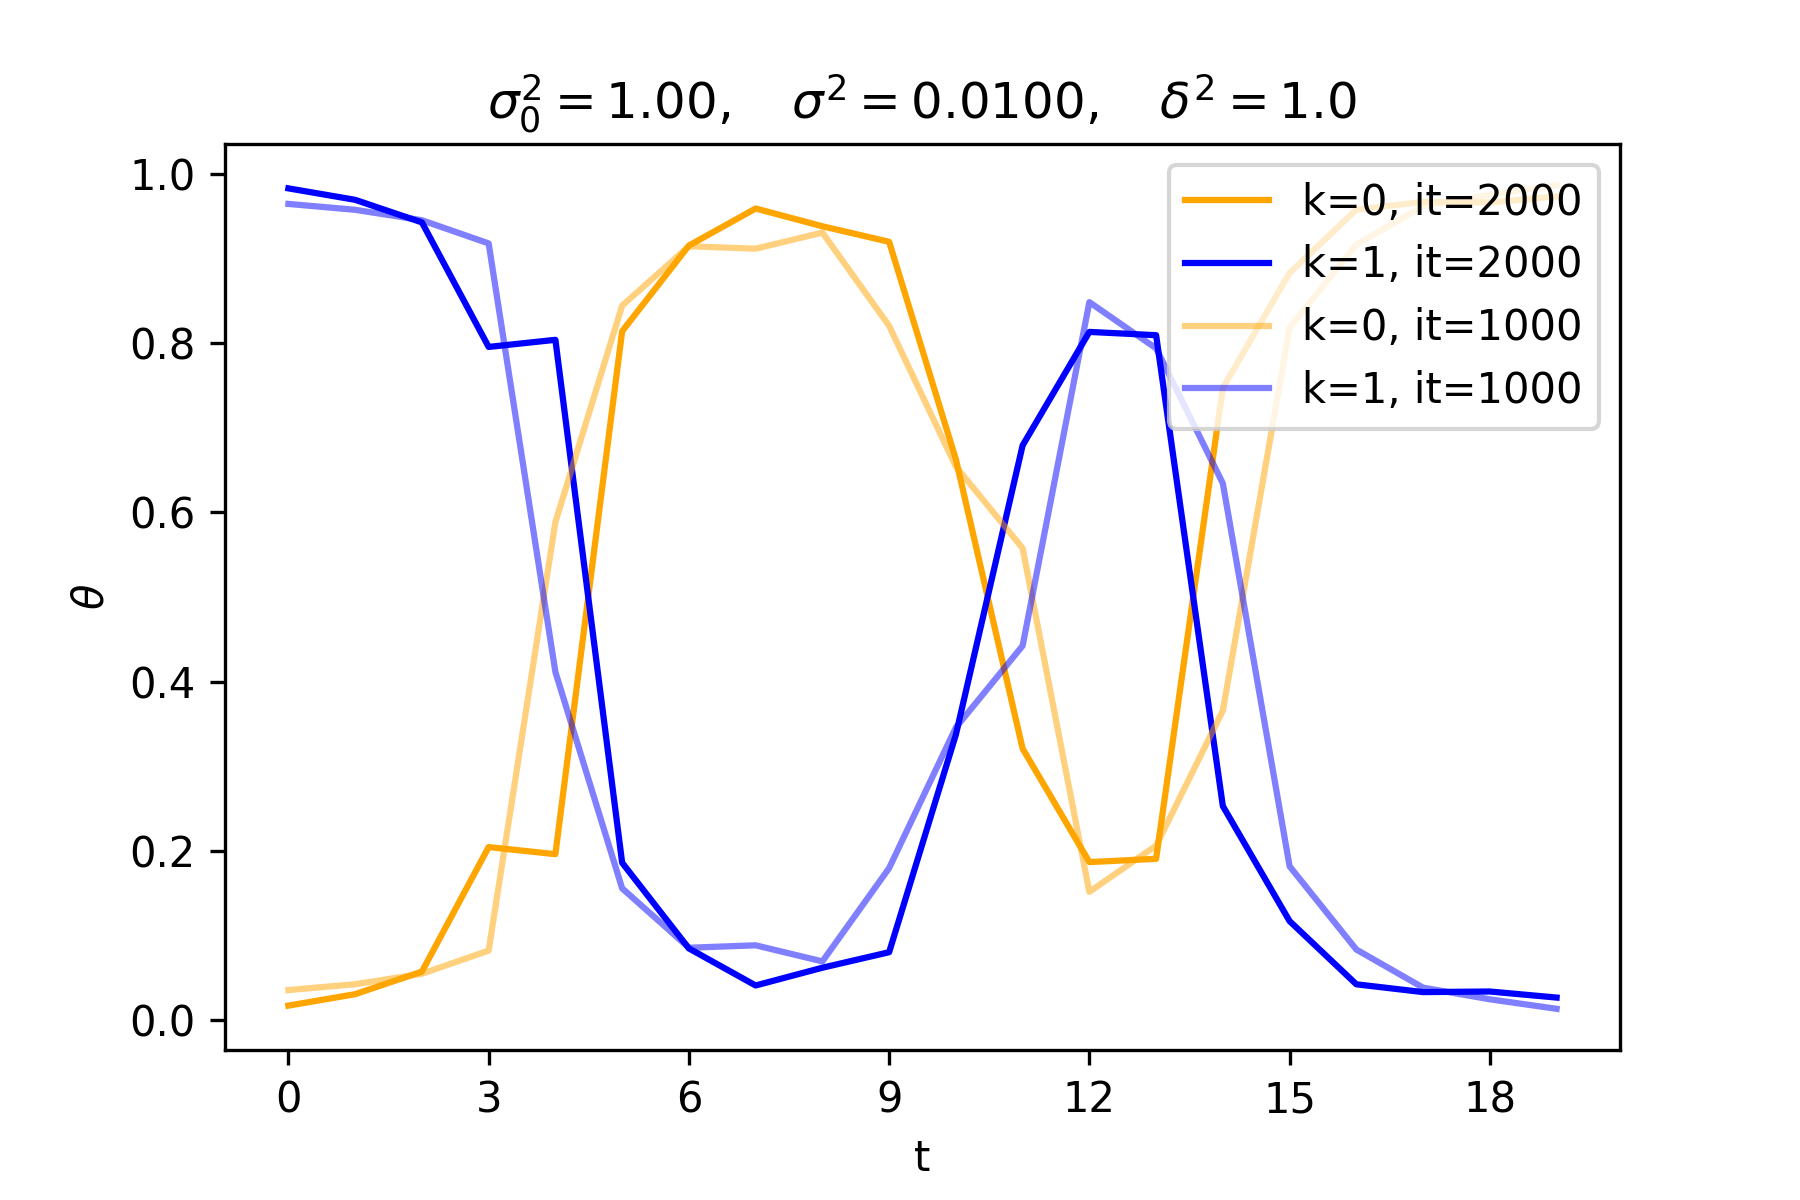
\includegraphics[width=\linewidth]{init_1E+00|basic_1E-02|prop_1E+00|it_2000|autoreg_True}
  \end{subfigure}%
  \begin{subfigure}[b]{0.33\textwidth}
    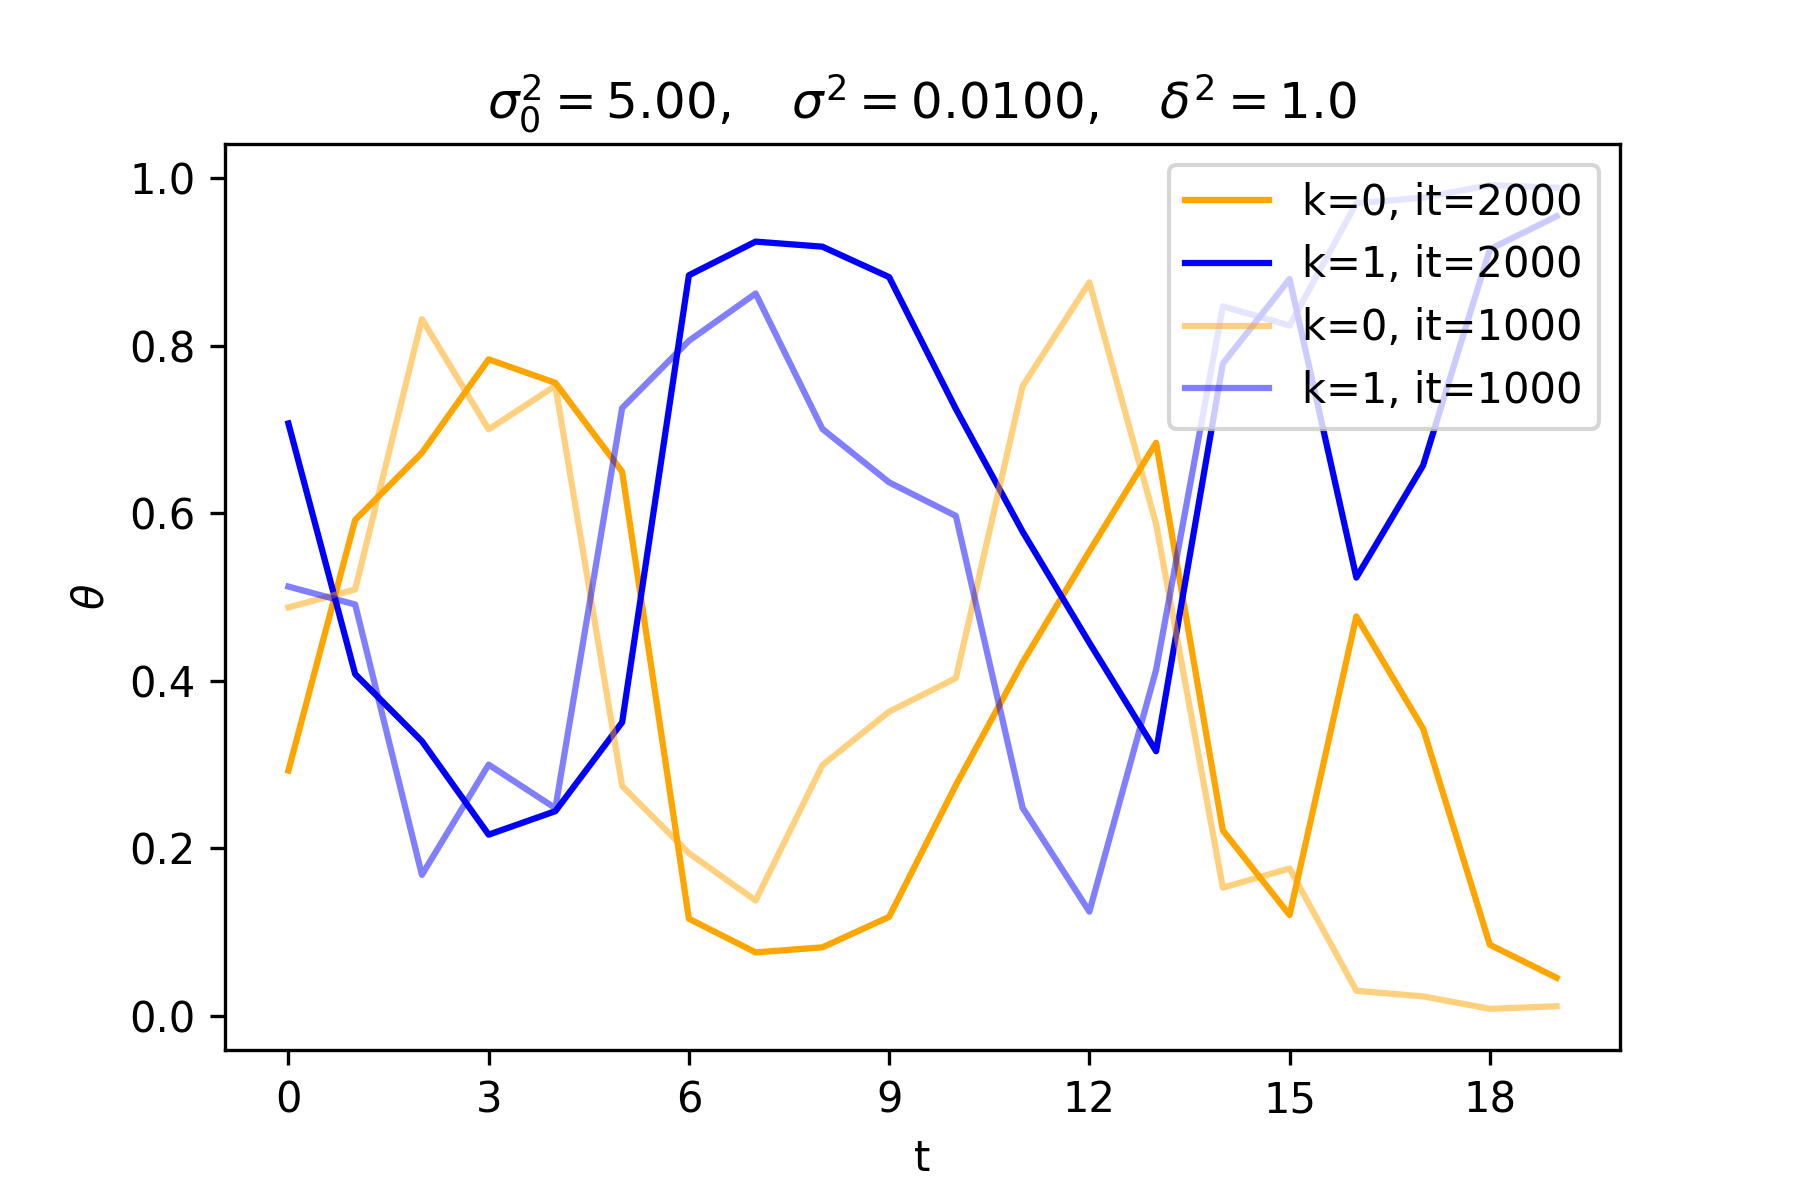
\includegraphics[width=\linewidth]{init_5E+00|basic_1E-02|prop_1E+00|it_2000|autoreg_True}
  \end{subfigure}
  \caption{Fixed $\sigma^2=0.01$.}
\end{figure}
\begin{figure}[H]
  \begin{subfigure}[b]{0.33\textwidth}
    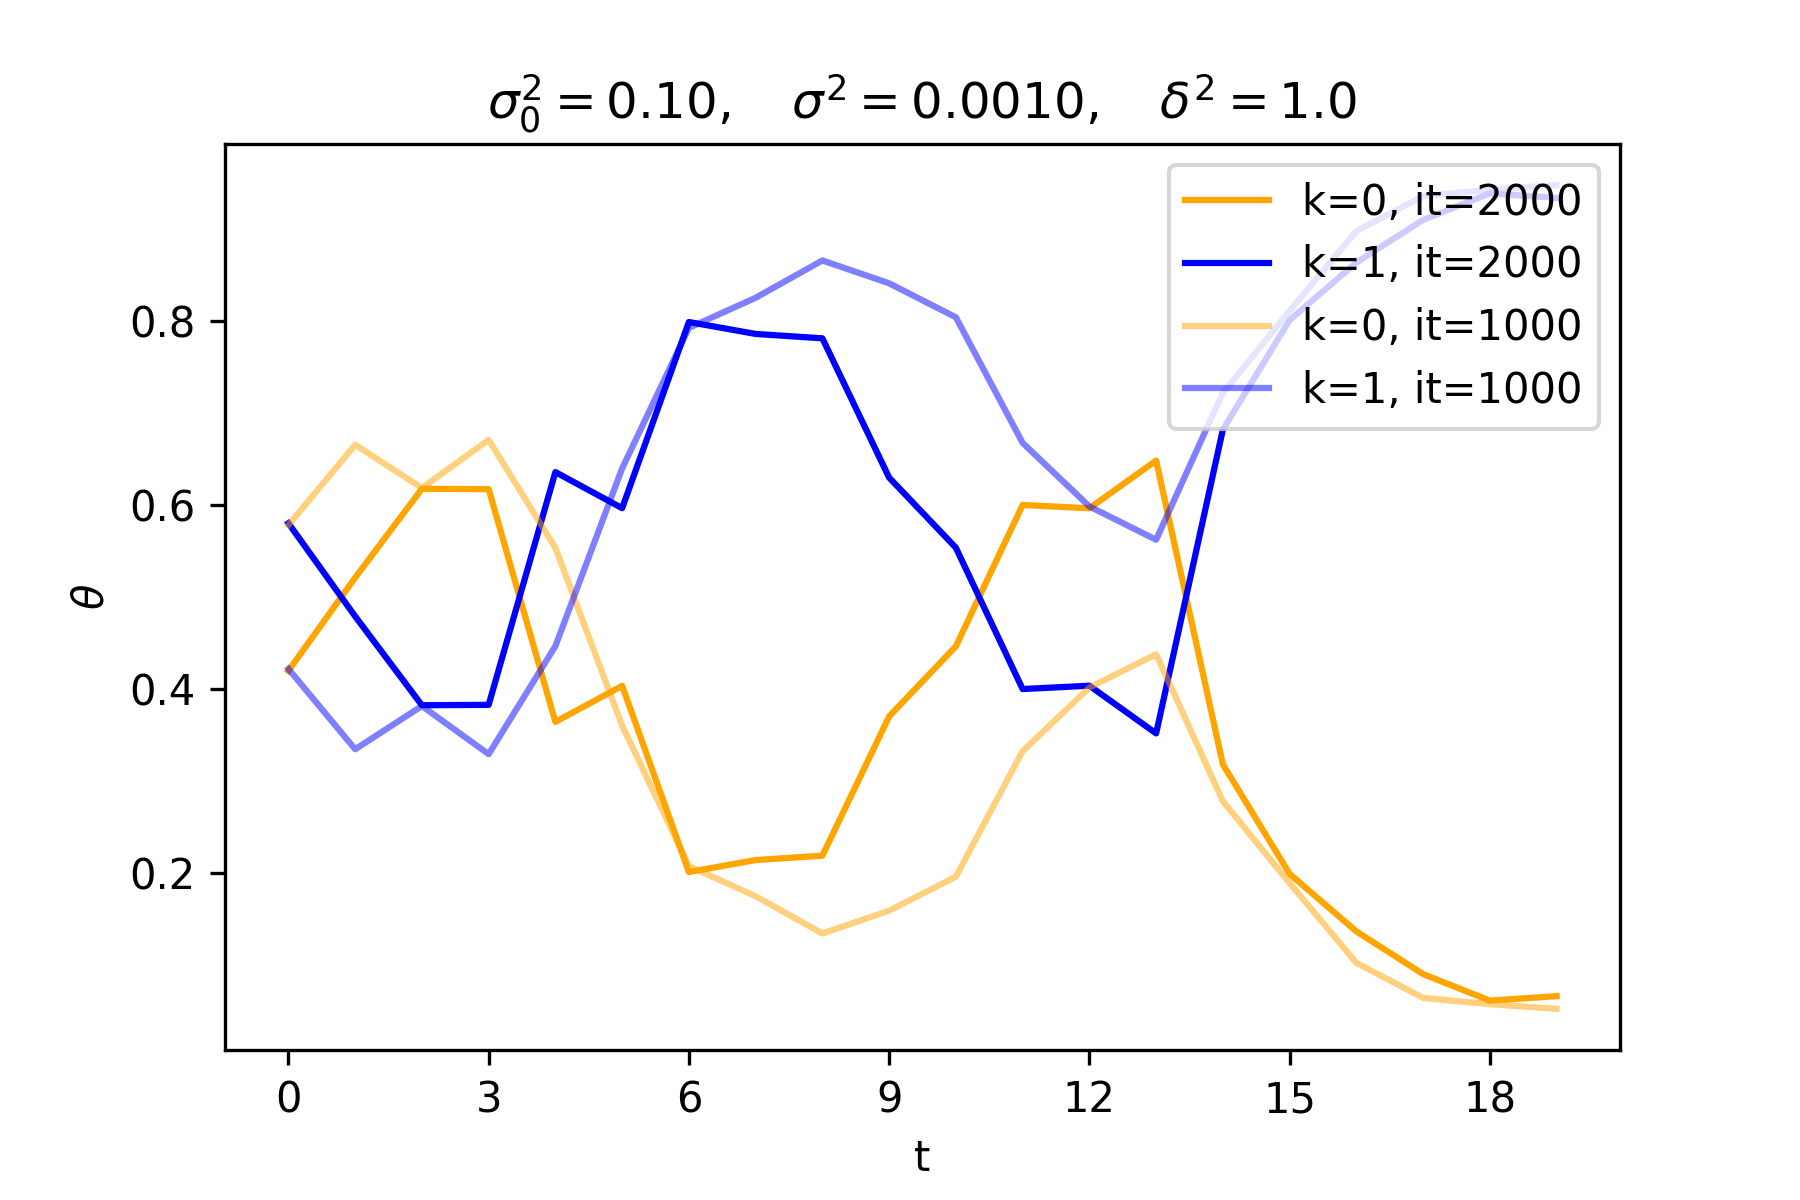
\includegraphics[width=\linewidth]{init_1E-01|basic_1E-03|prop_1E+00|it_2000|autoreg_True}
  \end{subfigure}%
  \begin{subfigure}[b]{0.33\textwidth}
    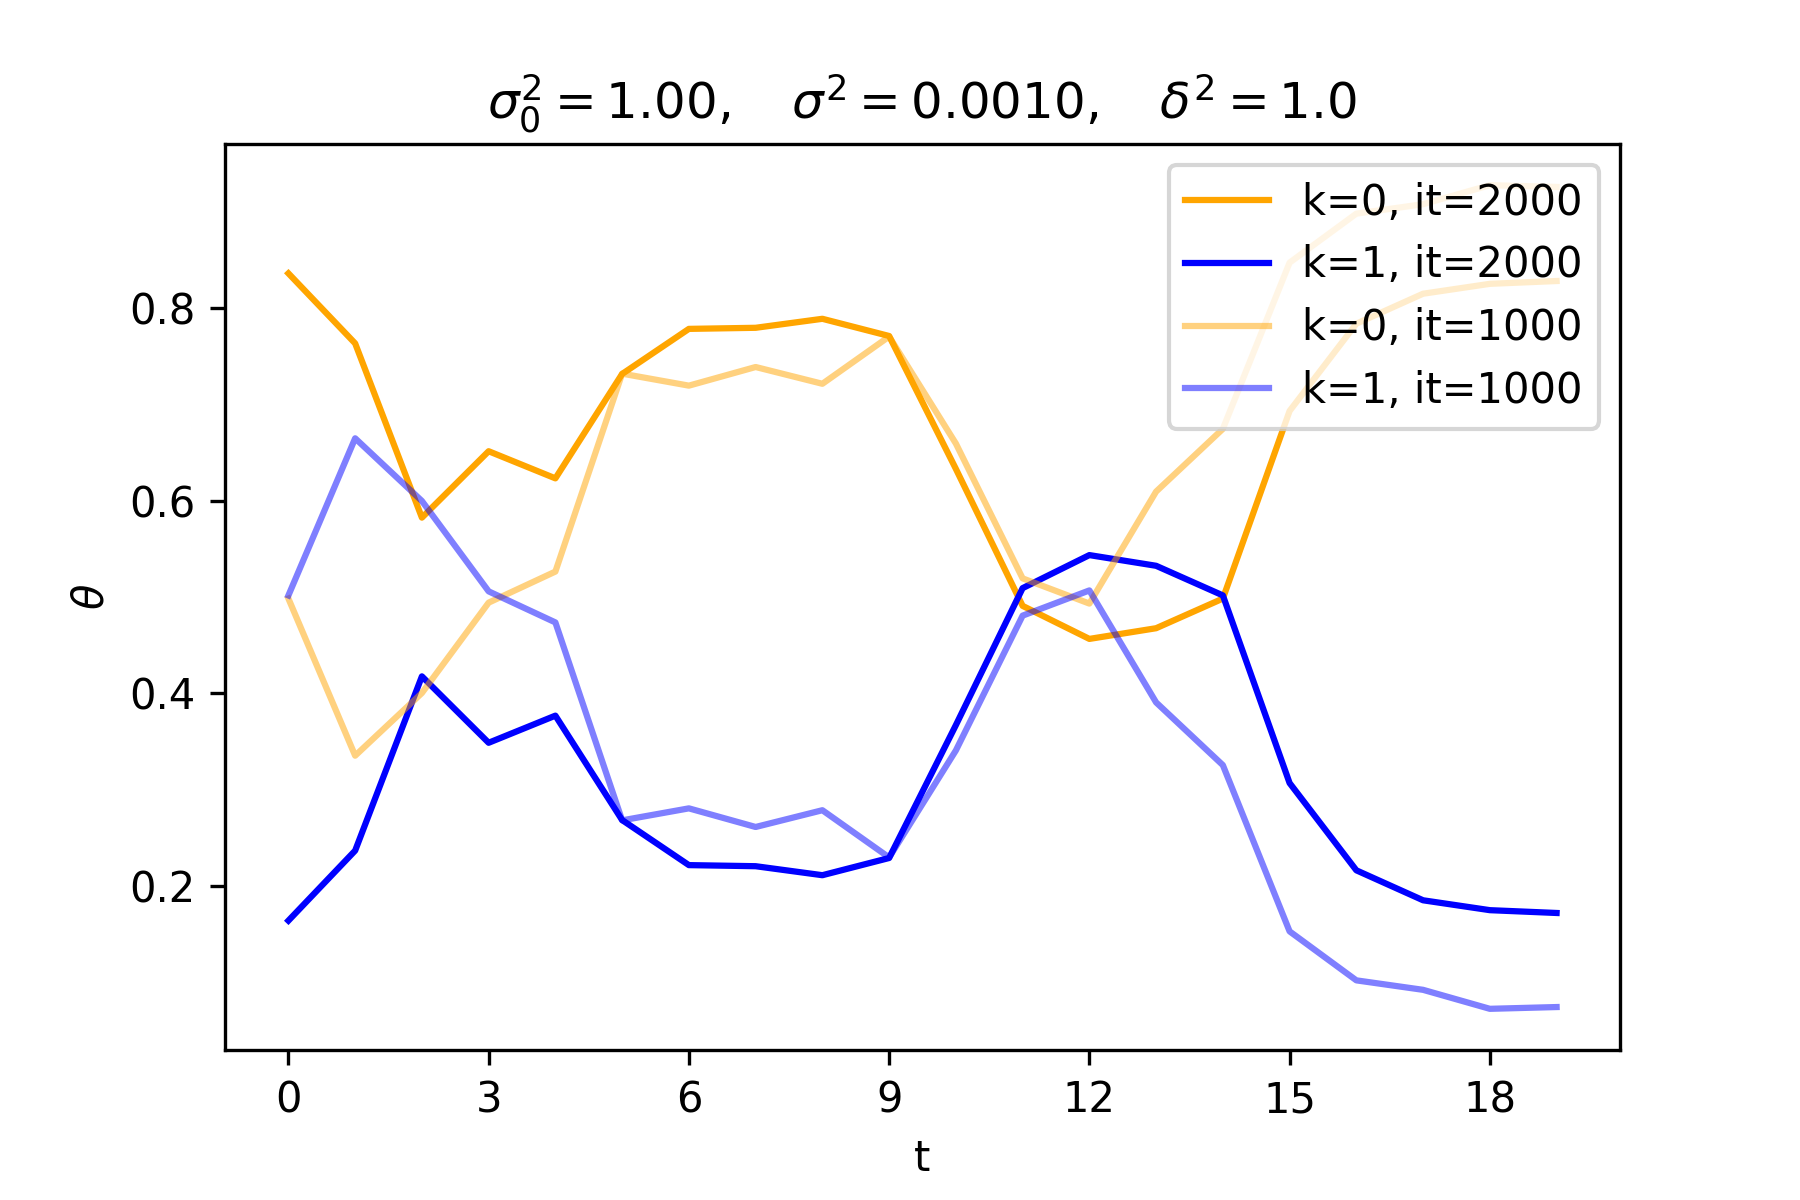
\includegraphics[width=\linewidth]{init_1E+00|basic_1E-03|prop_1E+00|it_2000|autoreg_True}
  \end{subfigure}%
  \begin{subfigure}[b]{0.33\textwidth}
    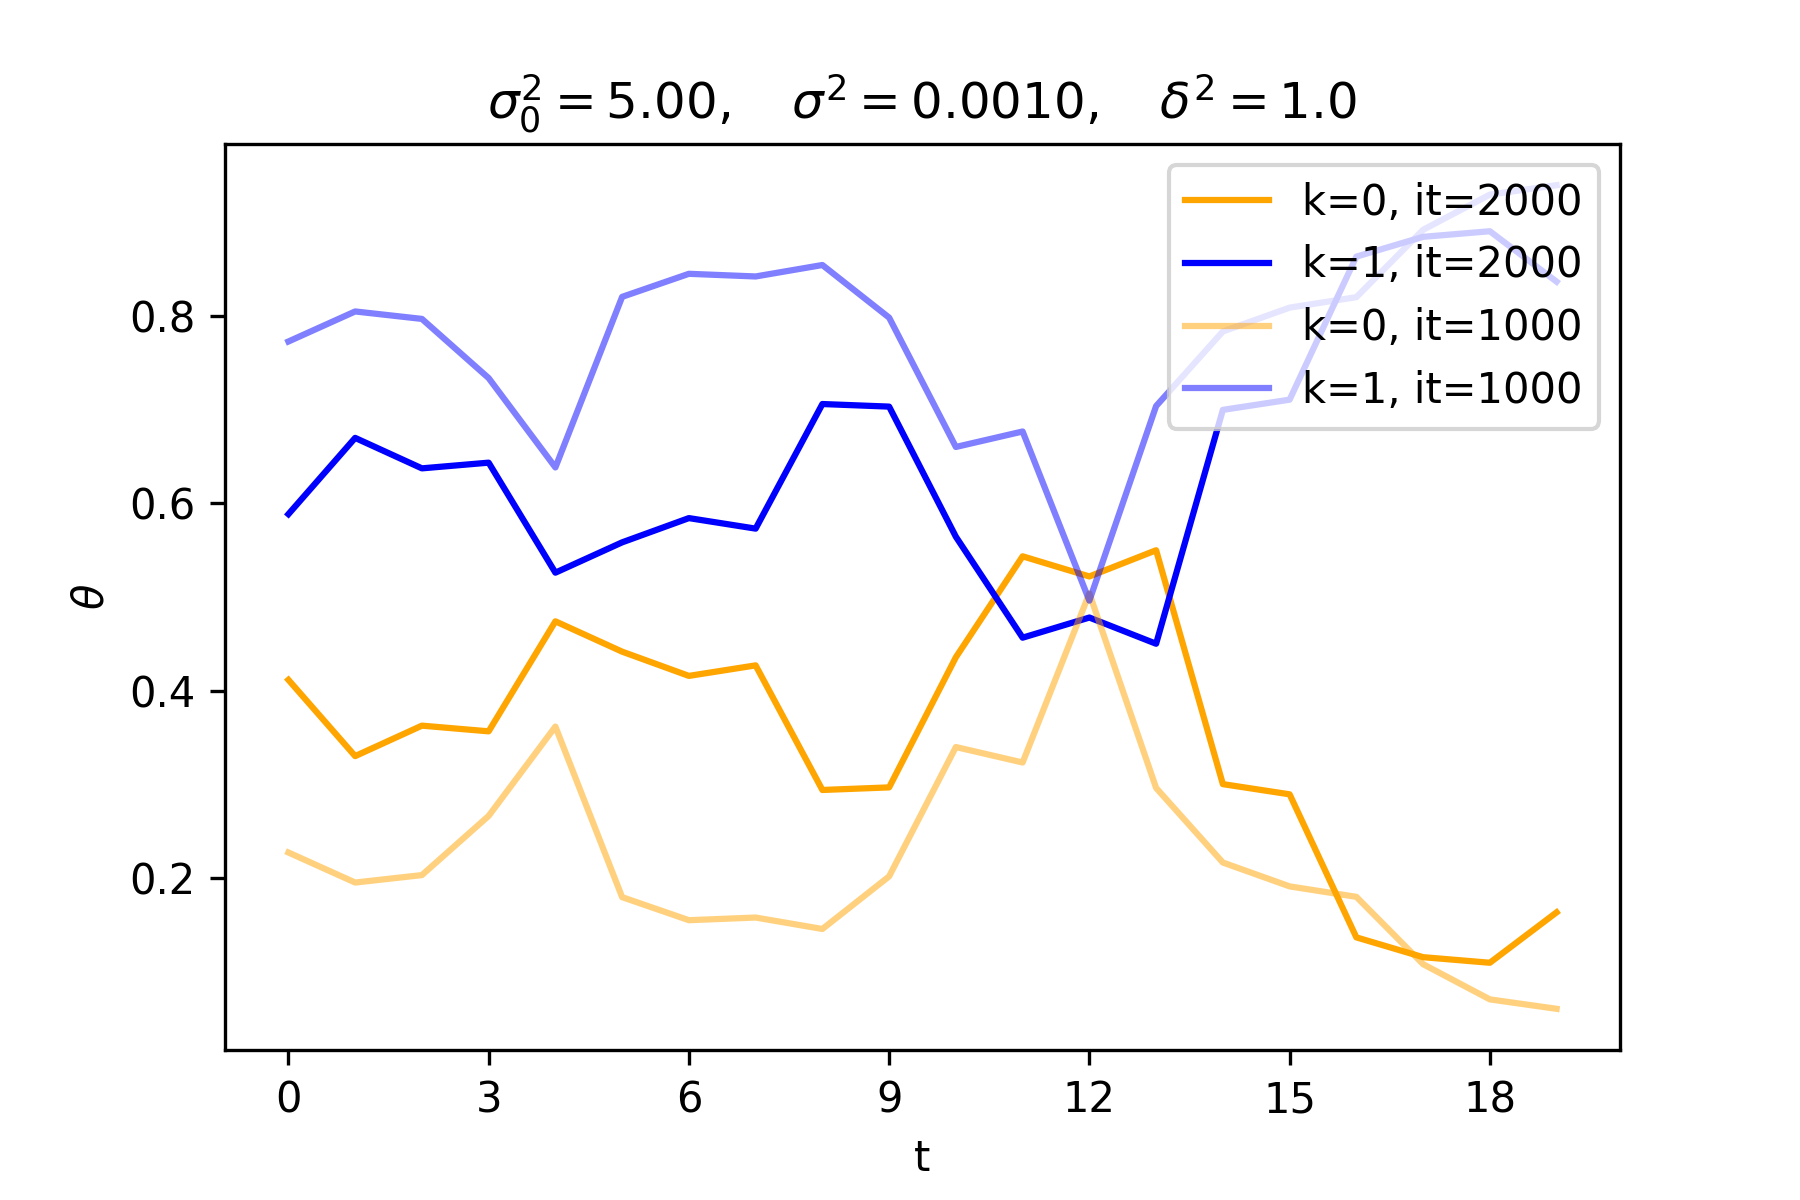
\includegraphics[width=\linewidth]{init_5E+00|basic_1E-03|prop_1E+00|it_2000|autoreg_True}
  \end{subfigure}
  \caption{Fixed $\sigma^2=0.001$.}
\end{figure}
\begin{figure}[H]
  \begin{subfigure}[b]{0.33\textwidth}
    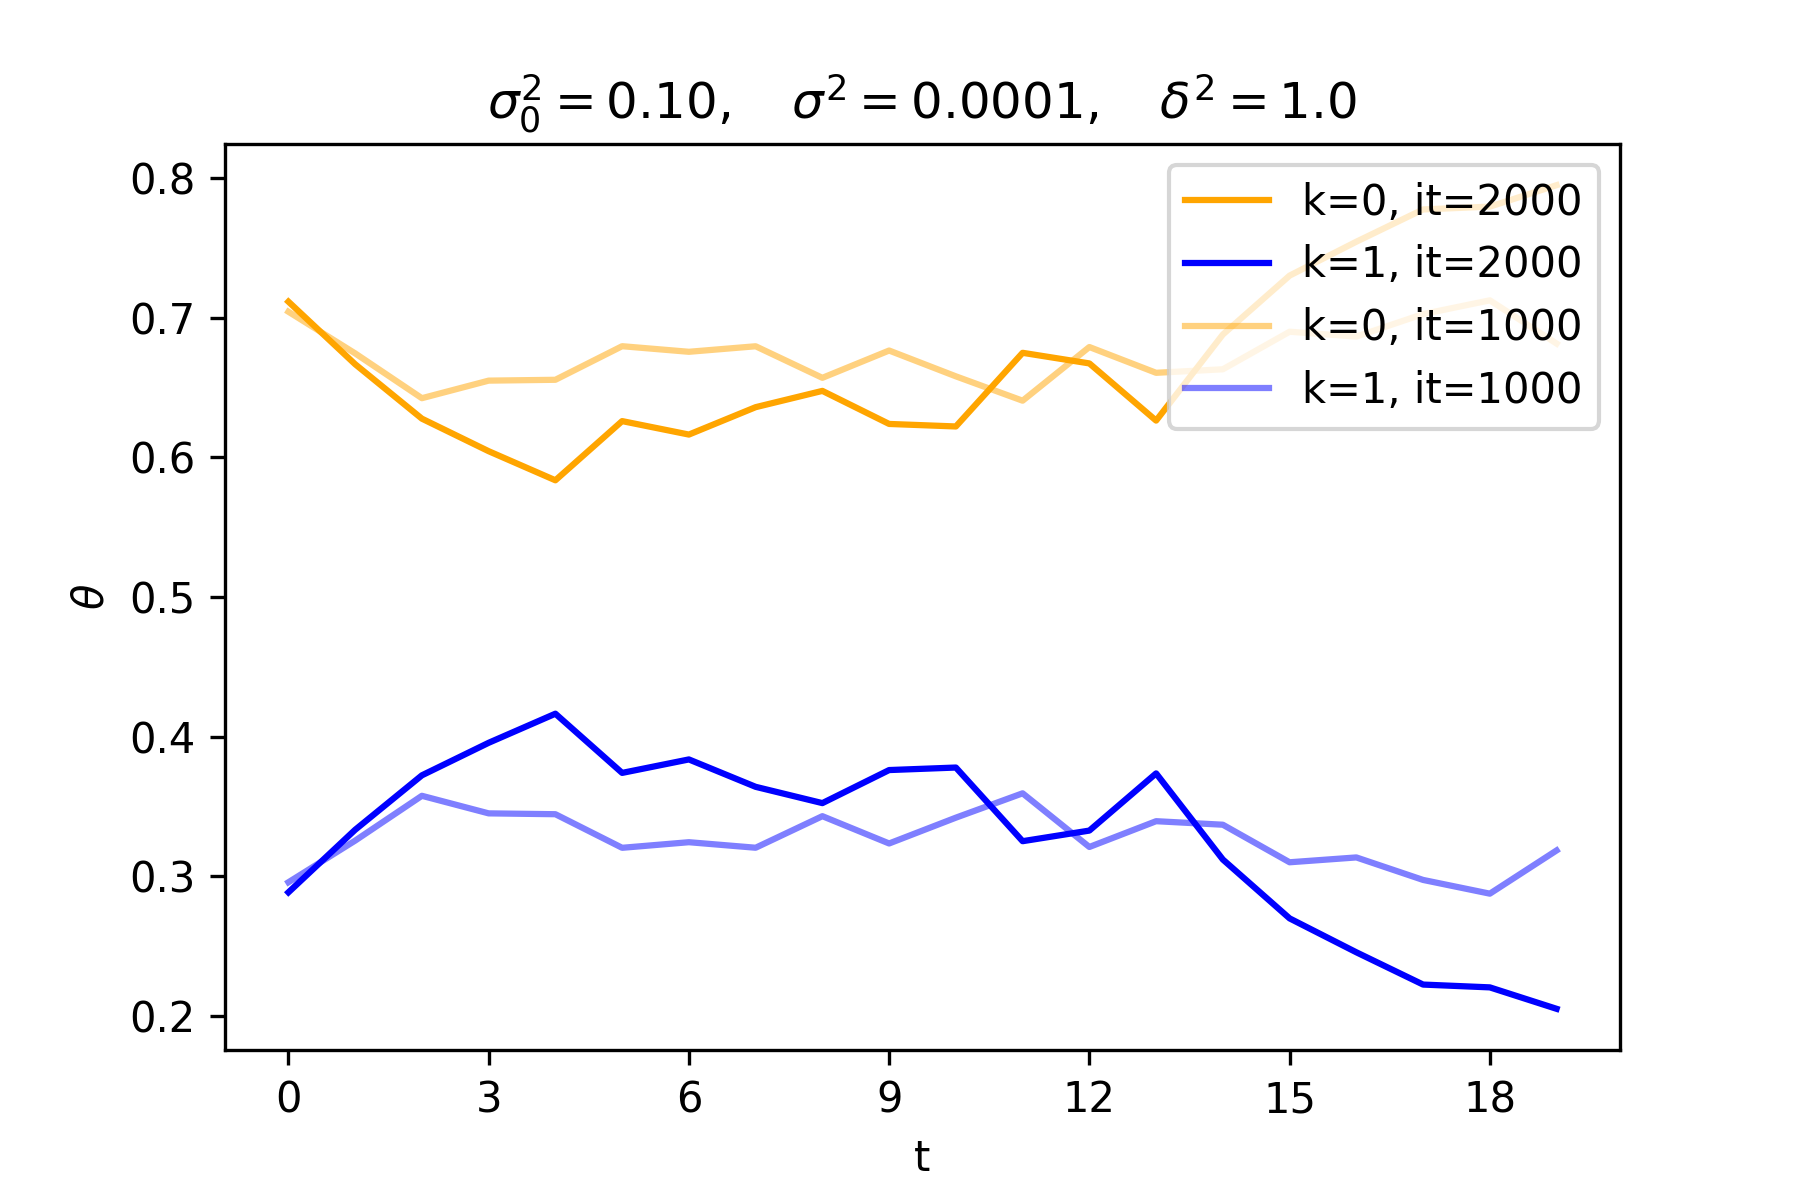
\includegraphics[width=\linewidth]{init_1E-01|basic_1E-04|prop_1E+00|it_2000|autoreg_True}
  \end{subfigure}%
  \begin{subfigure}[b]{0.33\textwidth}
    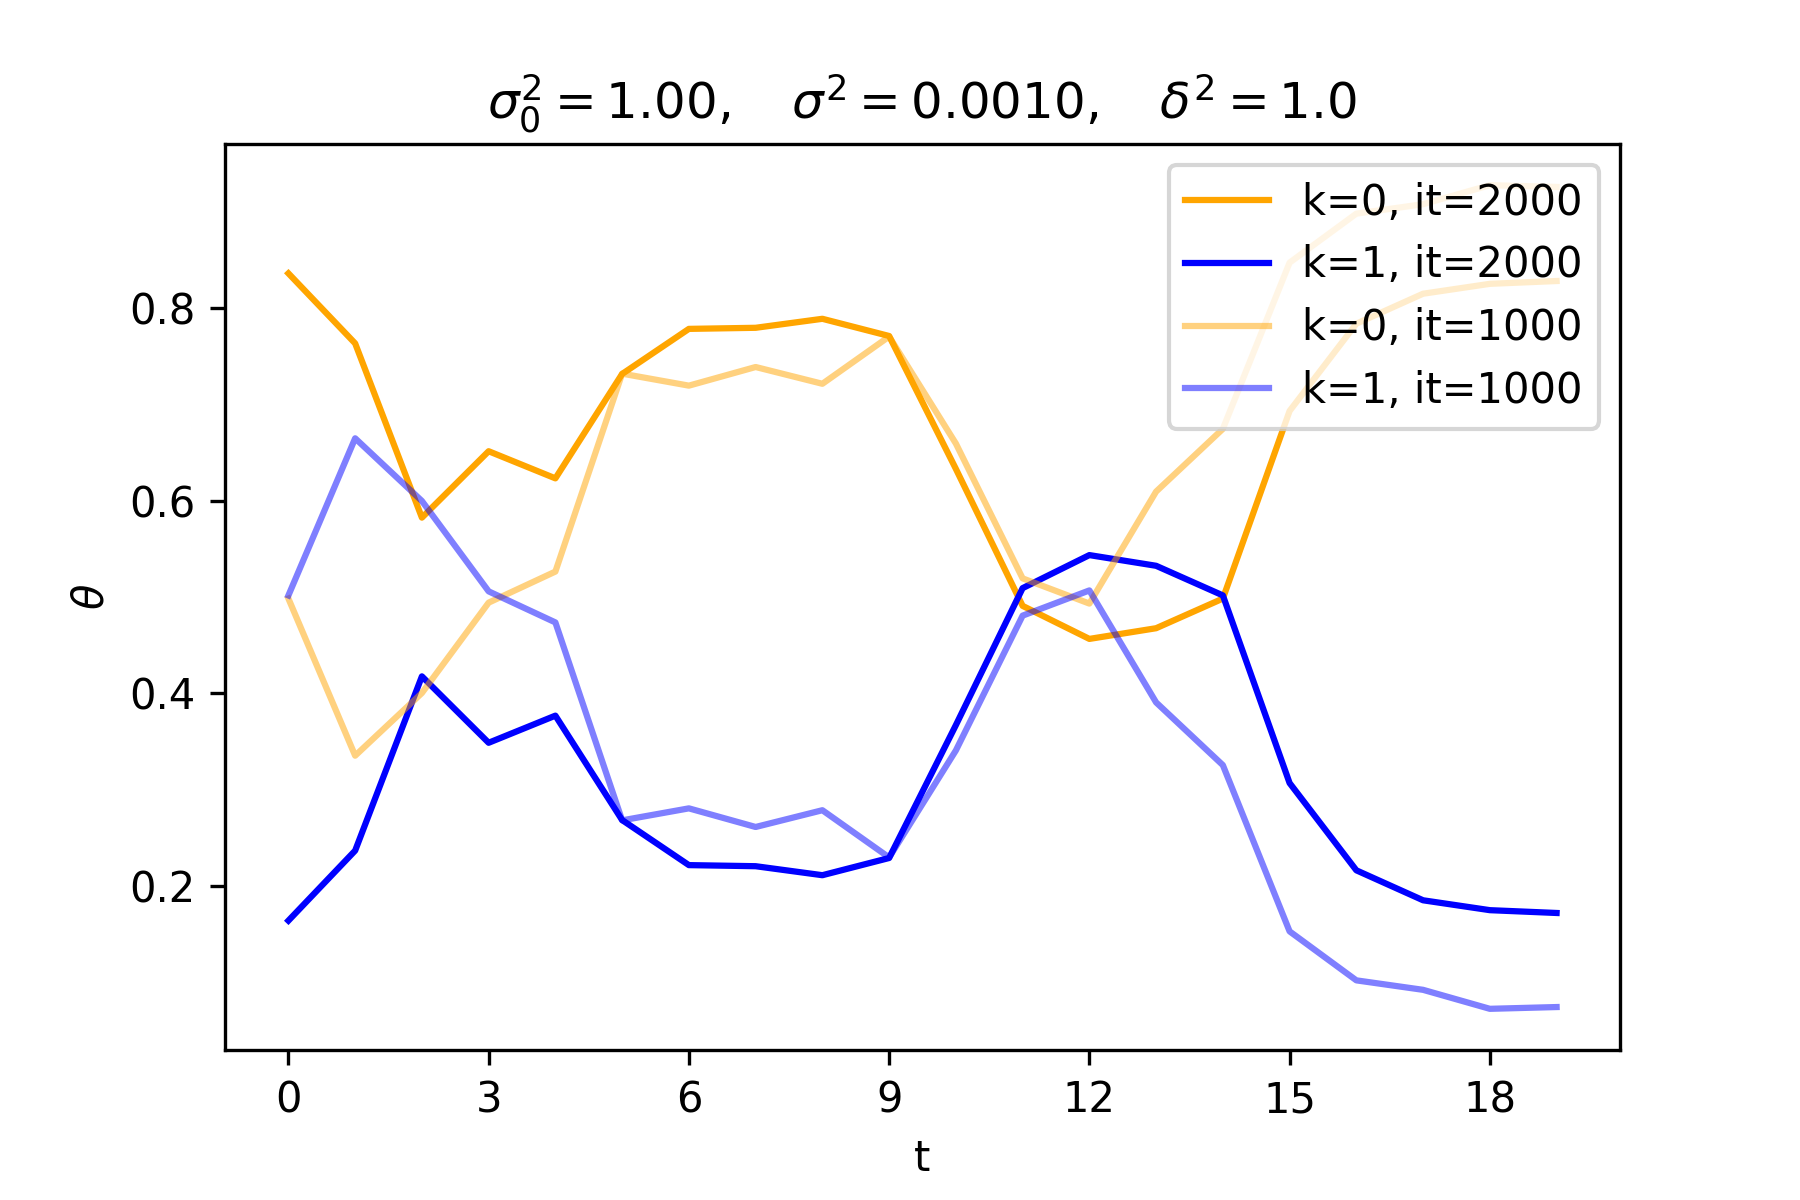
\includegraphics[width=\linewidth]{init_1E+00|basic_1E-03|prop_1E+00|it_2000|autoreg_True}
  \end{subfigure}%
  \begin{subfigure}[b]{0.33\textwidth}
    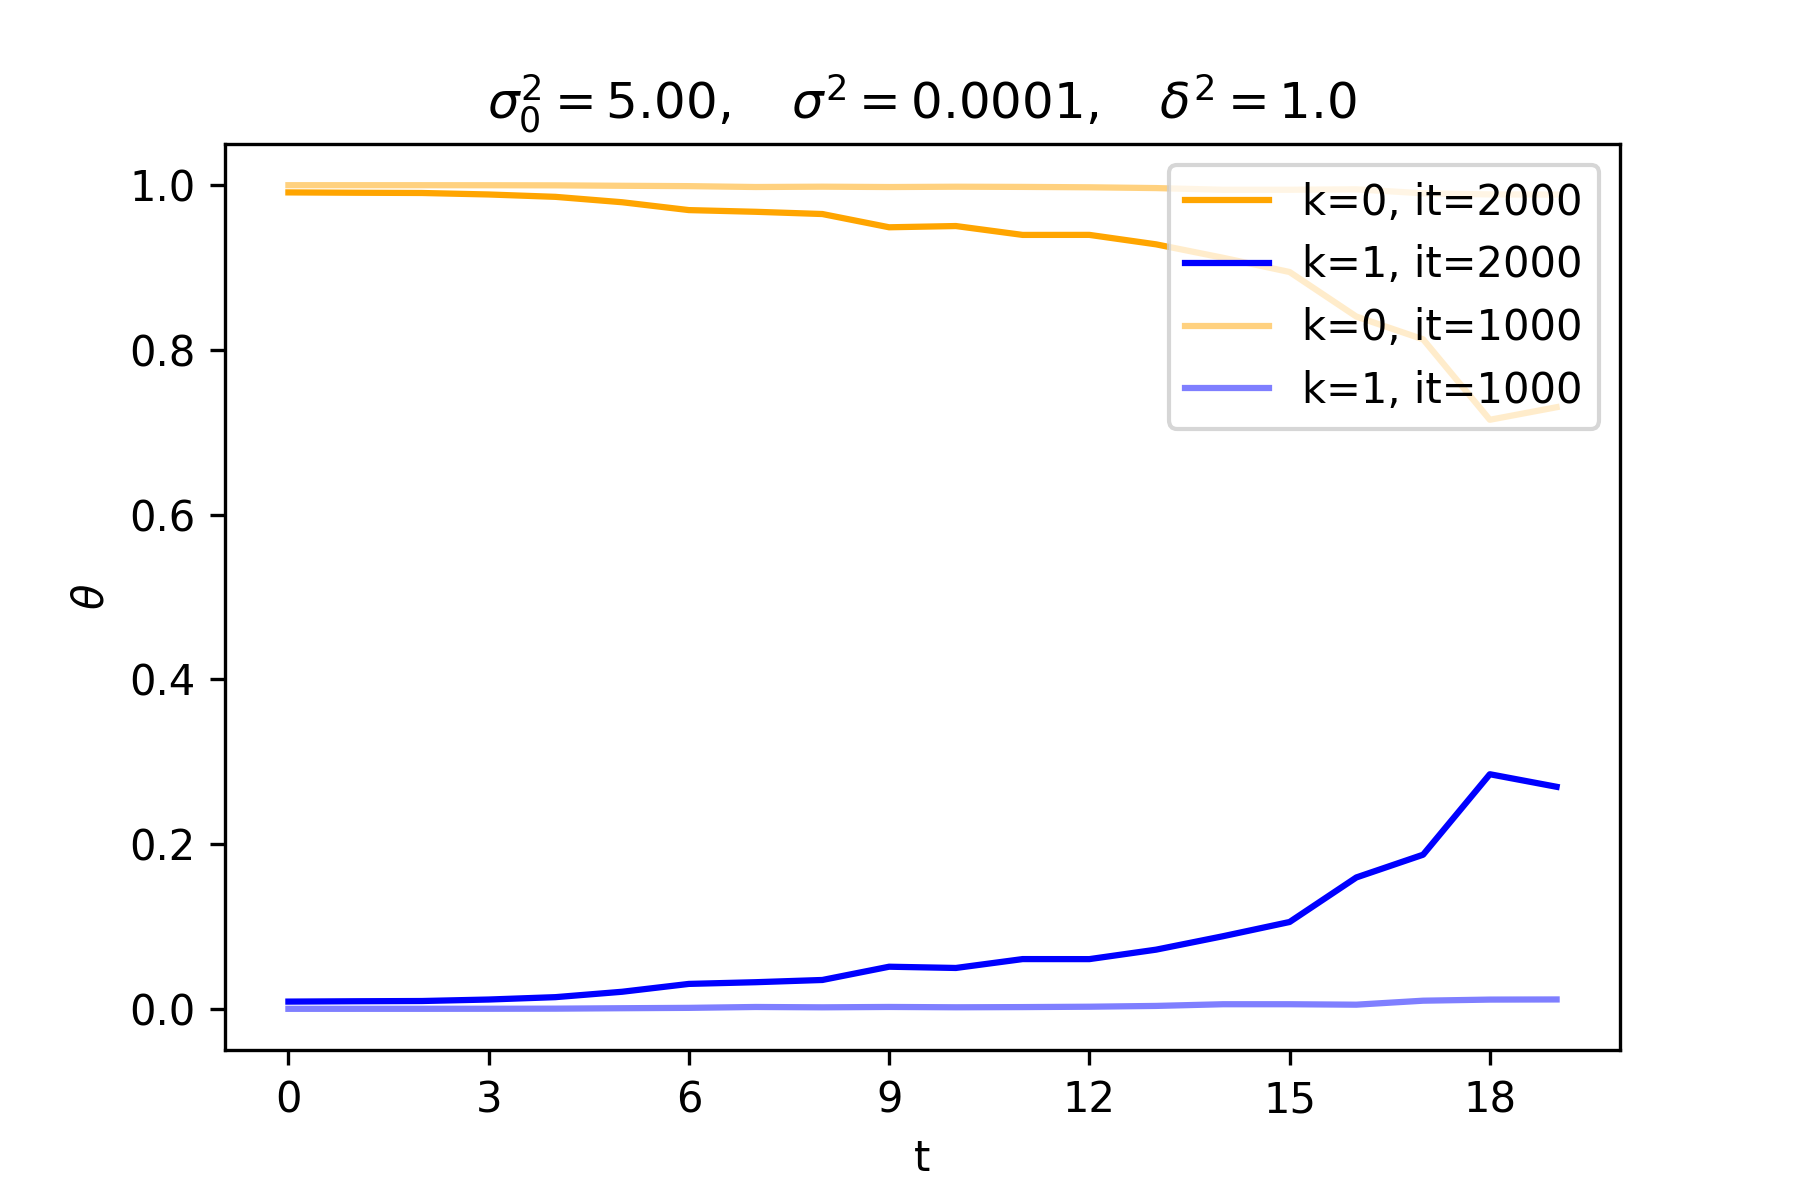
\includegraphics[width=\linewidth]{init_5E+00|basic_1E-04|prop_1E+00|it_2000|autoreg_True}
  \end{subfigure}
  \caption{Fixed $\sigma^2=0.0001$.}
\end{figure}

\par The second experiment assesses the impact of the auto-regressive $\alpha$ update. For this reason, the $\alpha$ prior was switched to the non auto-regressive one. Note that in this case $\sigma^2$ has no impact; therefore, we provide illustrations by varying the $\sigma^2_0$ term. Again, $\delta^2=1$ was kept constant throughout the experiments. Also, note that we ran the model for $200$ iterations. The resulting $\mbox{softmax}(\alpha)$ values are illustrated in Figure 6 below.

\begin{figure}[H]
  \begin{subfigure}[b]{0.33\textwidth}
    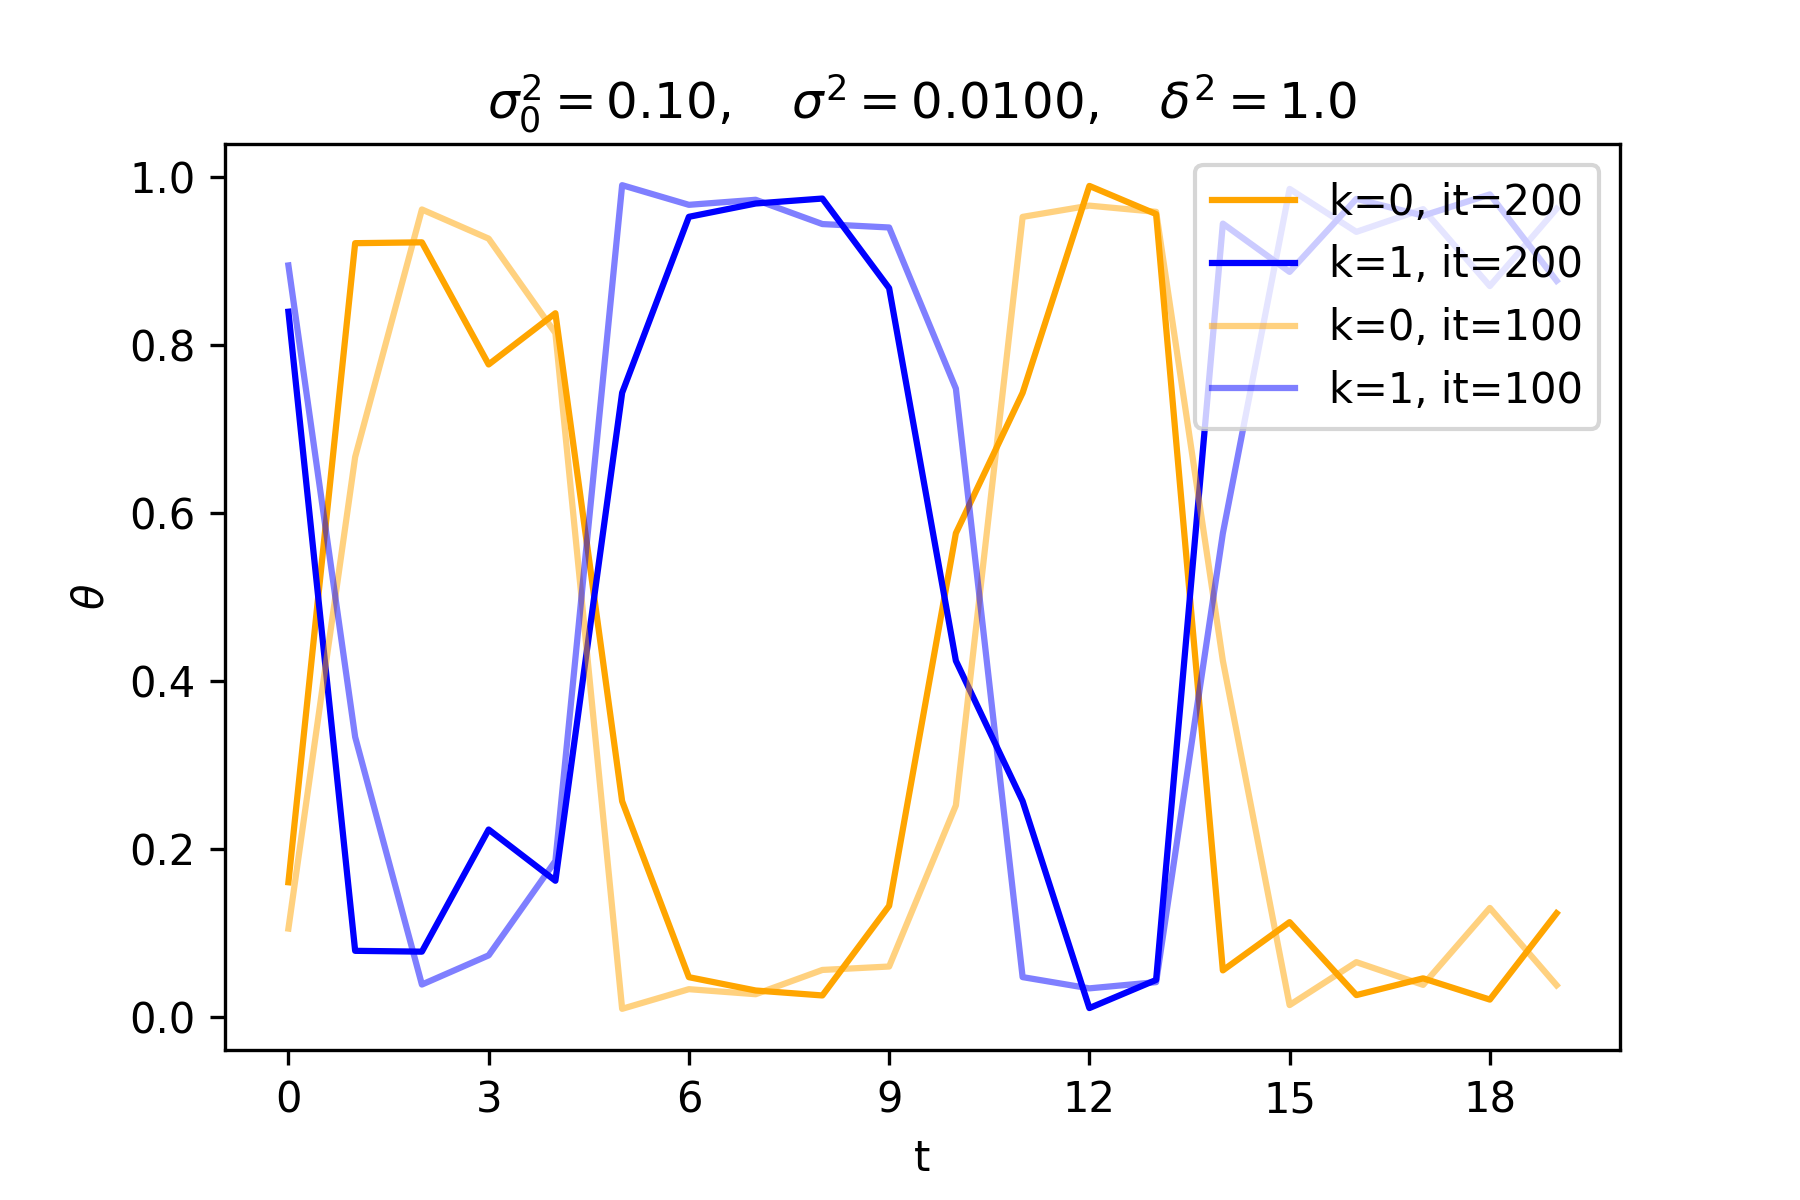
\includegraphics[width=\linewidth]{init_1E-01|basic_1E-02|prop_1E+00|it_200|autoreg_False}
  \end{subfigure}%
  \begin{subfigure}[b]{0.33\textwidth}
    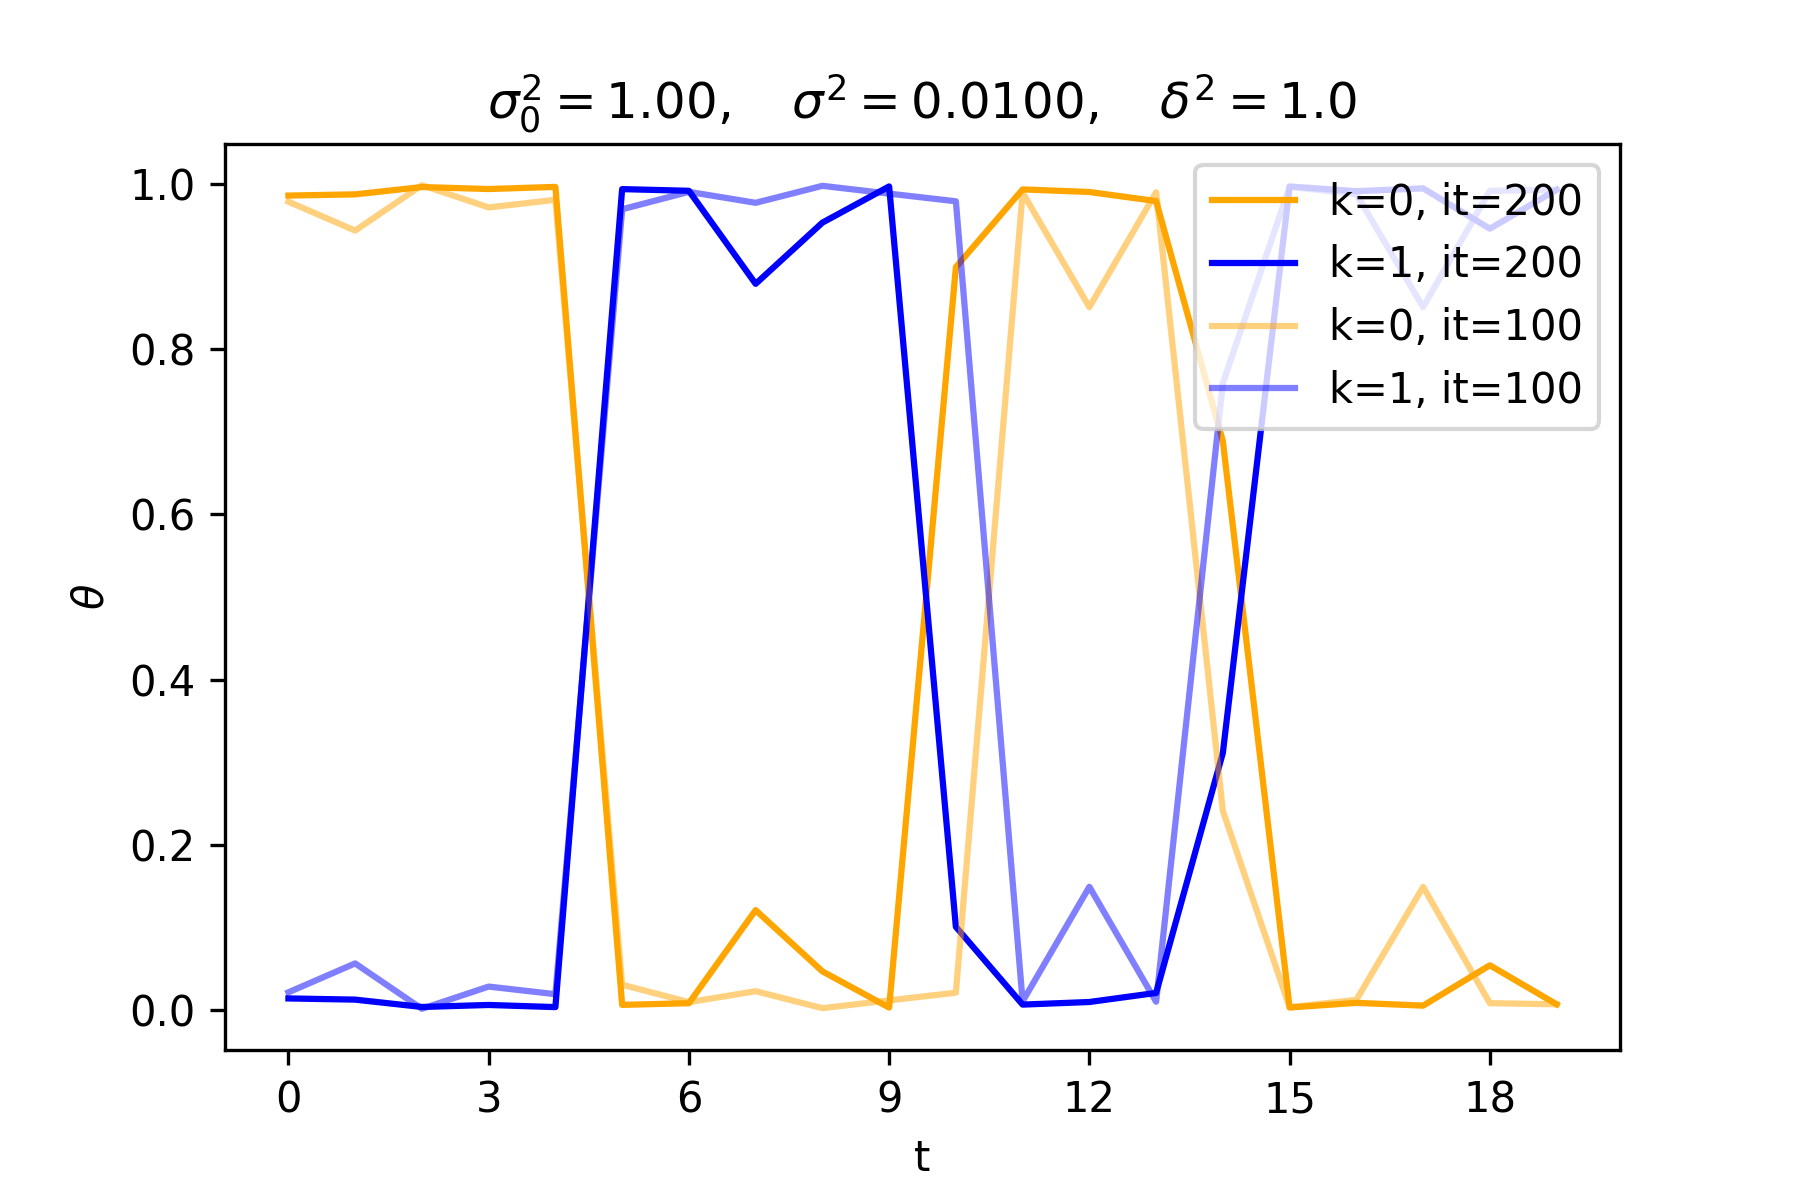
\includegraphics[width=\linewidth]{init_1E+00|basic_1E-02|prop_1E+00|it_200|autoreg_False}
  \end{subfigure}%
  \begin{subfigure}[b]{0.33\textwidth}
    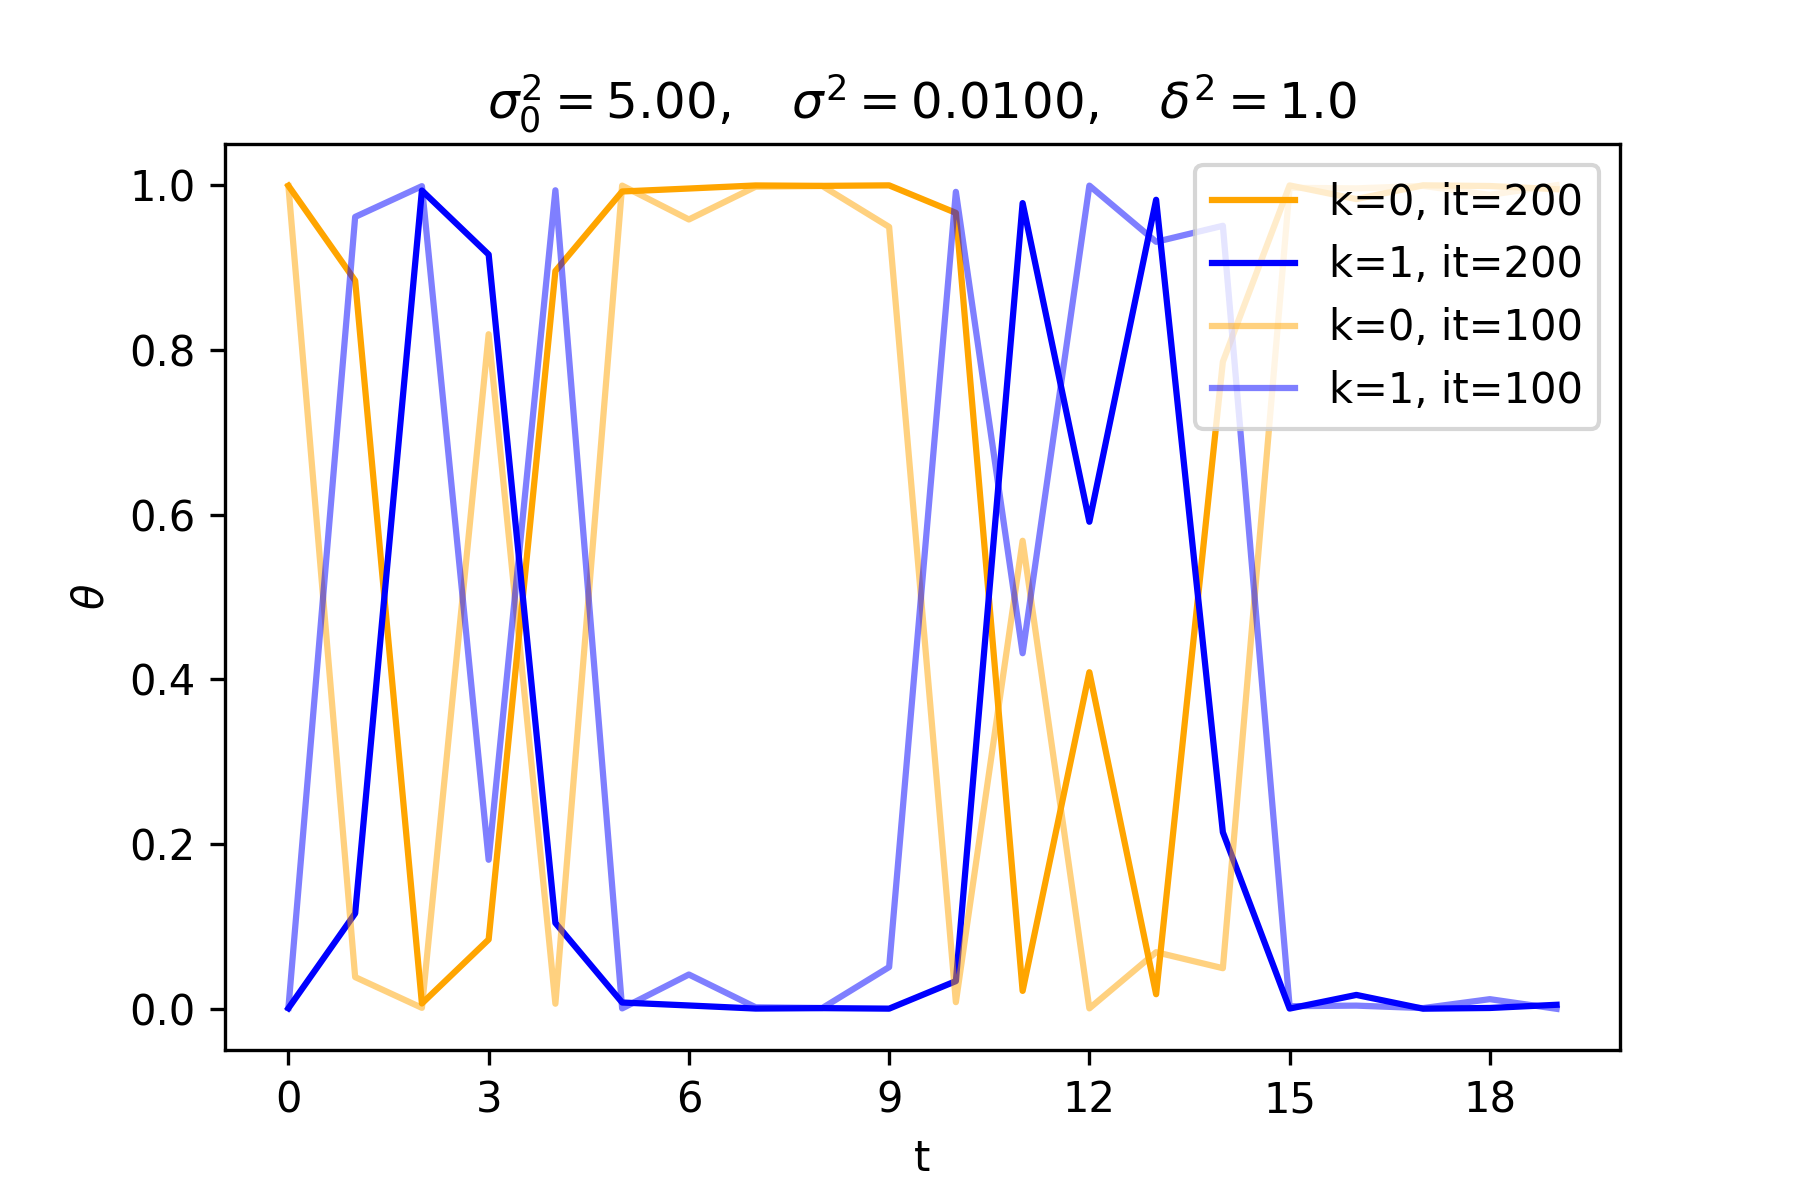
\includegraphics[width=\linewidth]{init_5E+00|basic_1E-02|prop_1E+00|it_200|autoreg_False}
  \end{subfigure}
  \caption{The non auto-regressive $\alpha$ update.}
\end{figure}
% ___________________________________________________________________

\section*{Questions}

\par For the last section of this report, I have set some questions to be addressed during next meeting; these are listed below:
\begin{itemize}
  \item During the derivation of the posterior given in Preliminaries Section, is the $\pi(\alpha_{t}')_k$ term, i.e. $p(z|\alpha^{-tk},\alpha_{t, k}')$, derived correctly? We did not have it explicitly expressed before.
  \item Should we consider the impact of tuning the model with the pre-defined $\beta$ (the one used during the synthetic corpus generation)? The model is able to recover the topic assignments to documents even if $\beta$ is initialised randomly. Also, do we have pre-defined $\beta$ for the non synthetic data sets?
  \item What are the indications of the faster $\alpha$ converge displayed in the non auto-regressive model? Could it mean that the model implementation is faulty?
\end{itemize}
% ___________________________________________________________________


%\bibliography{report_mh_alpha-update}{}
%\bibliographystyle{plain}
\end{document}
